\chapter{Modelli per le Emissioni Condotte}
L'emissione condotta identifica qualsiasi disturbo elettromagnetico in grado di propagarsi lungo strutture di interconnessione metalliche, quali le linee di alimentazione elettrica e le linee di trasmissione dati. A differenza delle emissioni irradiate, che si propagano nello spazio tridimensionale sotto forma di campi elettromagnetici liberi, le emissioni condotte viaggiano confinate all'interno dei conduttori fisici e si iniettano direttamente nella rete di distribuzione elettrica, potendo alterare il funzionamento di altri apparati connessi alla medesima infrastruttura.
\begin{figure}[H]
	\centering
	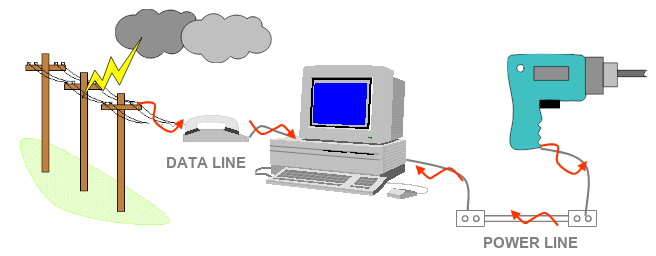
\includegraphics[width=0.7\linewidth]{immagini/emissioni_condotte1}
\end{figure}

L'intervallo di frequenza standard normato per la caratterizzazione delle emissioni condotte è compreso tra $150\text{ kHz}$ e $30\text{ MHz}$. La procedura per la verifica della conformità elettromagnetica si articola in due fasi sequenziali:
\begin{enumerate}
    \item Misurazione della tensione di disturbo presente ai capi dei conduttori di interconnessione, quantificata in decibel microvolt.
    \item Confronto dello spettro di tensione misurato con la maschera di limite imposta dalle normative vigenti in base alla destinazione d'uso dell'apparato.
\end{enumerate}

La quantificazione logaritmica della tensione di disturbo è definita dalla relazione:
\[
V_{\text{dB}\mu\text{V}} = 20 \log_{10}\left(\frac{V_{\text{misurata}}}{1\ \mu\text{V}}\right)
\]
dove $V_{\text{misurata}}$ rappresenta il valore efficace della tensione di rumore espresso in microvolt.

Le \textbf{norme internazionali CISPR 22 e FCC Part 15 Subpart J} prescrivono due classi di certificazione, a ciascuna delle quali corrisponde una specifica maschera limite di emissione valutata con rivelatore a quasi-picco:
\begin{itemize}
    \item \textbf{Classe A}, applicabile ad apparati destinati ad ambienti commerciali e industriali: prevede limiti meno restrittivi, con una soglia massima pari a $79\text{ dB}\mu\text{V}$ nella banda compresa tra $150\text{ kHz}$ e $500\text{ kHz}$, e pari a $73\text{ dB}\mu\text{V}$ nella banda compresa tra $500\text{ kHz}$ e $30\text{ MHz}$.
    \item \textbf{Classe B}, applicabile ad apparati destinati ad ambienti residenziali e domestici: impone vincoli più stringenti a tutela della rete civile, con un limite che parte da $66\text{ dB}\mu\text{V}$ a $150\text{ kHz}$ e decresce linearmente con il logaritmo della frequenza fino a $56\text{ dB}\mu\text{V}$ a $500\text{ kHz}$, si mantiene costante a $56\text{ dB}\mu\text{V}$ nell'intervallo compreso tra $500\text{ kHz}$ e $5\text{ MHz}$, e si stabilizza a $60\text{ dB}\mu\text{V}$ tra $5\text{ MHz}$ e $30\text{ MHz}$.
\end{itemize}
\begin{figure}[H]
	\centering
	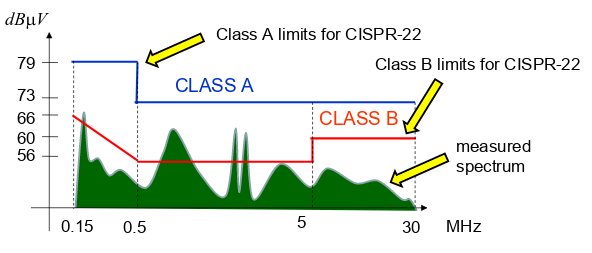
\includegraphics[width=0.7\linewidth]{immagini/emissioni_condotte2}
\end{figure}
Il contenimento delle emissioni condotte entro la soglia di Classe B costituisce il requisito di progetto prioritario per gli apparati commerciali.

\section{Misurazione delle emissioni condotte}
La misurazione delle emissioni condotte richiede la determinazione delle tensioni di disturbo presenti sulla linea di fase $V_P$ e sulla linea di neutro $V_N$, rilevate su resistori puri da $50\ \Omega$ rispetto al conduttore di protezione a massa. La medesima configurazione si applica a qualunque altra linea di interconnessione, incluse le linee di trasmissione dati. 
\begin{figure}[H]
	\centering
	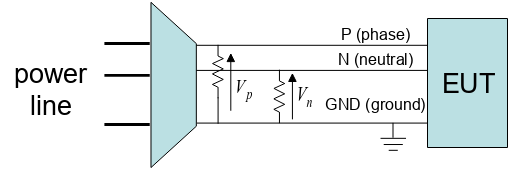
\includegraphics[width=0.6\linewidth]{immagini/emissioni_condotte3}
\end{figure}
L'esecuzione di tale misura direttamente sulla rete di alimentazione presenta due criticità fondamentali:
\begin{itemize}
    \item \textbf{Dipendenza dall'impedenza di linea} $\rightarrow$ l'impedenza interna della rete di distribuzione non presenta un valore noto né costante, variando continuamente in funzione dell'ora del giorno, della lunghezza delle tratte di cavo e degli altri carichi collegati all'impianto; di conseguenza, la tensione di disturbo misurata ai morsetti dell'EUT varierebbe in modo non ripetibile tra diversi laboratori di prova.
    \item \textbf{Presenza di rumore di fondo esterno} $\rightarrow$ la tensione rilevata ai morsetti includerebbe non solo i disturbi originati internamente dall'EUT, ma anche il rumore condotto proveniente dalla rete elettrica esterna e dalla cabina di trasformazione, impedendo di caratterizzare in modo univoco il dispositivo sotto esame.
\end{itemize}

\subsection{Rete di stabilizzazione dell'impedenza di linea (LISN)}
Per superare i problemi di non riproducibilità legati alla variabilità della rete e isolare il contributo di disturbo dell'apparato sotto test, tra la rete di alimentazione e l'EUT viene inserita la \textbf{LISN (Line Impedance Stabilization Network)}.
\begin{figure}[H]
	\centering
	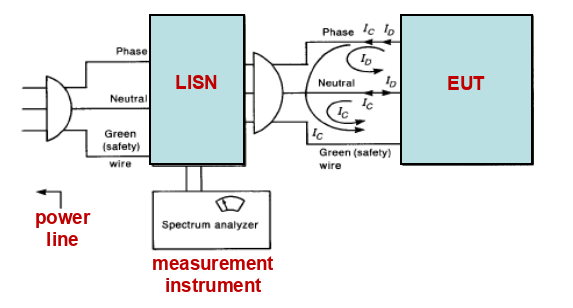
\includegraphics[width=0.6\linewidth]{immagini/emissioni_condotte4}
\end{figure}
La LISN adempie a tre funzioni operative fondamentali:
\begin{itemize}
    \item \textbf{Stabilizzazione dell'impedenza di linea} $\rightarrow$ presenta un'impedenza calibrata e costante, pari a $50\ \Omega$, tra ciascun conduttore attivo e la massa metallica di riferimento in tutto l'intervallo di frequenza compreso tra $150\text{ kHz}$ e $30\text{ MHz}$.
    \item \textbf{Disaccoppiamento e filtraggio della rete} $\rightarrow$ attenua e devia verso massa i disturbi ad alta frequenza provenienti dalla rete elettrica esterna, impedendo che si sovrappongano alla misura.
    \item \textbf{Trasparenza alla frequenza di rete} $\rightarrow$ consente il transito della corrente di alimentazione alla frequenza nominale di $50\text{ Hz}$ con caduta di potenziale e dissipazione trascurabili.
\end{itemize}

Lo schema circuitale della LISN impiega componenti reattivi dimensionati per esibire comportamenti duali alle frequenze di lavoro:
\begin{itemize}
    \item \textbf{$C_{in} = 1\ \mu F$} $\rightarrow$ condensatori di ingresso collegati tra fase e massa e tra neutro e massa sul lato collegato alla rete di alimentazione.
    \item \textbf{$L_{serie} = 50\ \mu H$} $\rightarrow$ induttori inseriti in serie sulle linee di fase e di neutro tra la sezione di ingresso e la sezione di misura.
    \item \textbf{$C_{out} = 0.1\ \mu F$} $\rightarrow$ condensatori di accoppiamento e blocco in continua interposti tra le linee di segnale e i morsetti di prelievo della strumentazione.
    \item \textbf{$R_{int} = 1k\Omega$} $\rightarrow$ resistori interni di polarizzazione connessi stabilmente tra ciascuna linea di segnale e la massa di riferimento.
    \item \textbf{$R_L = 50\Omega$} $\rightarrow$ impedenza di ingresso del ricevitore di misura o carico fittizio di chiusura a $50\ \Omega$, collegato in parallelo al resistore da $1\text{ k}\Omega$ sulla porta non utilizzata per preservare il bilanciamento circuitale.
\end{itemize}
\begin{figure}[H]
	\centering
	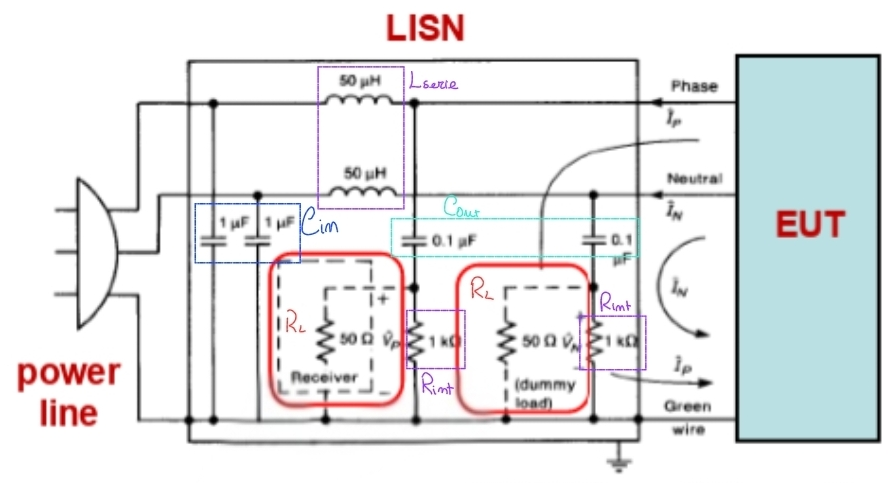
\includegraphics[width=0.7\linewidth]{immagini/emissioni_condotte5}
\end{figure}
In condizioni operative di misura, la presenza del resistore da $1\text{ k}\Omega$ in parallelo al carico da $50\ \Omega$ determina un'impedenza equivalente vista dall'EUT pari a:
\[
R_{eq} = \frac{50 \cdot 1000}{50 + 1000} \approx 47.6\ \Omega \approx 50\ \Omega
\]
La deviazione rispetto al valore nominale di $50\ \Omega$ risulta inferiore al $5\%$, rientrando nelle tolleranze di misura previste dagli standard.

Nell'intervallo normato compreso tra $150\text{ kHz}$ e $30\text{ MHz}$, i componenti reattivi soddisfano i seguenti vincoli di impedenza rispetto al riferimento di $50\ \Omega$:
\[
Z_C = \frac{1}{\omega C} \ll 50\ \Omega
\]
\[
Z_L = \omega L \gg 50\ \Omega
\]
In questa banda:
\begin{itemize}
    \item I condensatori d'ingresso da $1\ \mu\text{F}$ presentano un'impedenza trascurabile e agiscono come cortocircuiti verso massa, deviando integralmente il rumore proveniente dalla linea di rete e mascherandone l'impedenza.
    \item Gli induttori in serie da $50\ \mu\text{H}$ presentano un'impedenza elevata e agiscono come circuiti aperti, bloccando la propagazione di correnti di disturbo tra la rete e la sezione di test.
    \item I condensatori di accoppiamento da $0.1\ \mu\text{F}$ agiscono come cortocircuiti, trasferendo le tensioni di disturbo generate dall'EUT direttamente sui resistori di misura da $50\ \Omega$.
\end{itemize}
Il circuito equivalente risultante ad alta frequenza vede l'EUT terminato unicamente su due resistenze pure da $50\ \Omega$ connesse verso il conduttore di protezione a massa. 
\begin{figure}[H]
	\centering
	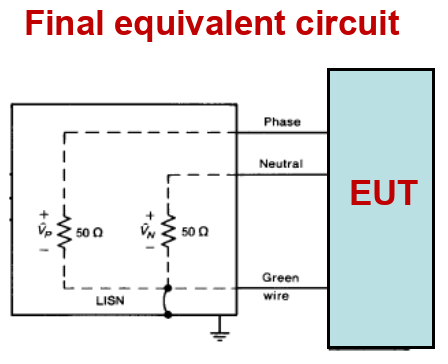
\includegraphics[width=0.4\linewidth]{immagini/emissioni_condotte6}
\end{figure}
Le tensioni misurate risultano legate alle correnti di linea dalle relazioni ai fasori:
\[
\hat{V}_P = 50 \hat{I}_P
\]
\[
\hat{V}_N = 50 \hat{I}_N
\]
dove $\hat{I}_P$ e $\hat{I}_N$ indicano i fasori della corrente di fase e di neutro uscenti dall'EUT verso la LISN.

Alla frequenza nominale di alimentazione di $50\text{ Hz}$, i componenti reattivi invertono il rispettivo regime di funzionamento:
\[
Z_C = \frac{1}{\omega C} \gg 50\ \Omega
\]
\[
Z_L = \omega L \ll 50\ \Omega
\]
\newpage
Nello specifico:
\begin{itemize}
    \item I condensatori da $1\ \mu\text{F}$ agiscono come circuiti aperti, non assorbendo corrente reattiva dalla rete.
    \item Gli induttori da $50\ \mu\text{H}$ agiscono come cortocircuiti, lasciando scorrere la corrente di potenza verso l'EUT senza cadute di tensione apprezzabili.
    \item I condensatori da $0.1\ \mu\text{F}$ operano come circuiti aperti, isolando e proteggendo i ricevitori di misura dalla tensione di rete a $50\text{ Hz}$.
\end{itemize}
Il circuito equivalente a $50\text{ Hz}$ coincide con la connessione diretta e trasparente dell'EUT alla rete elettrica di alimentazione:
\begin{figure}[H]
	\centering
	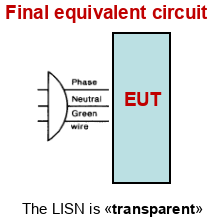
\includegraphics[width=0.35\linewidth]{immagini/emissioni_condotte7}
\end{figure}

\subsection{Correnti di modo comune e modo differenziale}
L'individuazione delle cause dei disturbi condotti e la progettazione dei rimedi circuitali richiedono la scomposizione delle correnti misurate su fase e neutro in due componenti ortogonali:
\begin{itemize}
    \item \textbf{$\hat{I}_D$} $\rightarrow$ \textbf{corrente di modo differenziale} che scorre lungo la linea di fase e si richiude in senso opposto lungo il neutro, formando una spira confinata tra i due conduttori attivi senza coinvolgere il conduttore di terra.
    \item \textbf{$\hat{I}_C$} $\rightarrow$ \textbf{corrente di modo comune} che fluisce nello stesso verso su entrambi i conduttori di fase e neutro, trovando il proprio percorso di ritorno verso la sorgente attraverso il conduttore di protezione a massa.
\end{itemize}
\begin{figure}[H]
	\centering
	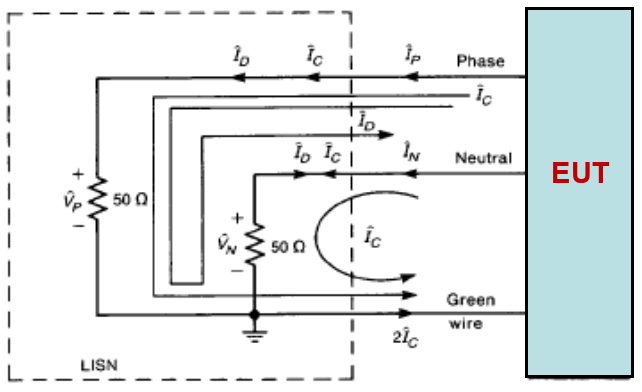
\includegraphics[width=0.5\linewidth]{immagini/emissioni_condotte8}
\end{figure}
Le correnti totali di linea sui conduttori di fase e neutro sono espresse dalla sovrapposizione delle due modalità:
\[
\hat{I}_P = \hat{I}_C + \hat{I}_D
\]
\[
\hat{I}_N = \hat{I}_C - \hat{I}_D
\]
Invertendo il sistema lineare si ottengono le espressioni per l'estrazione delle singole componenti:
\[
\hat{I}_D = \frac{1}{2}(\hat{I}_P - \hat{I}_N)
\]
\[
\hat{I}_C = \frac{1}{2}(\hat{I}_P + \hat{I}_N)
\]

Le tensioni rilevate dalla LISN sui resistori di carico da $50\ \Omega$ connessi tra ciascun conduttore e la massa assumono la formulazione:
\[
\hat{V}_P = 50(\hat{I}_C + \hat{I}_D)
\]
\[
\hat{V}_N = 50(\hat{I}_C - \hat{I}_D)
\]

La distribuzione spettrale delle due componenti lungo l'intervallo compreso tra $150\text{ kHz}$ e $30\text{ MHz}$ manifesta comportamenti distinti:
\begin{figure}[H]
	\centering
	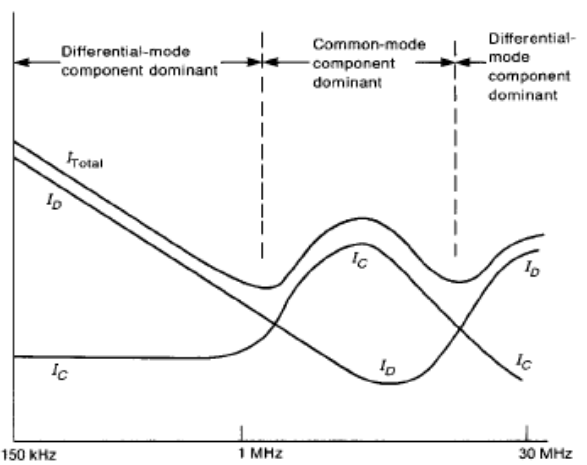
\includegraphics[width=0.4\linewidth]{immagini/emissioni_condotte9}
\end{figure}
\begin{itemize}
    \item Basse frequenze ($< 1\text{ MHz}$): domina la componente di modo differenziale $\hat{I}_D$, generata dalla corrente funzionale assorbita dal carico e dalle correnti di ripple di commutazione degli stadi di potenza.
    \item Alte frequenze ($> 1\text{ MHz}$): domina la componente di modo comune $\hat{I}_C$, la quale cresce rapidamente a causa delle correnti capacitive parassite che scavalcano l'isolamento e si richiudono sul telaio metallico di massa in presenza di elevate derivate di potenziale; il modo comune costituisce la causa principale del mancato rispetto delle maschere normative oltre $1\text{ MHz}$.
    \item Frequenze prossime a $30\text{ MHz}$: l'insorgenza di risonanze parassite può dar luogo a incrementi secondari anche nella componente differenziale residua.
\end{itemize}

\section{Sorgenti di disturbo per emissioni condotte}
I disturbi condotti originano primariamente dagli stadi di conversione negli apparati elettronici. Vediamo il confronto tra le due principali topologie di alimentatori:
\begin{itemize}
    \item \textbf{Alimentatori lineari}: impiegano un trasformatore a $50\text{ Hz}$, un ponte raddrizzatore e un transistor che opera in regione attiva con funzione di regolatore. Generano livelli di emissione condotta ridotti per l'assenza di commutazioni veloci, ma soffrono di bassa efficienza ed elevata dissipazione termica sul transistor di potenza.
    \begin{figure}[H]
    	\centering
    	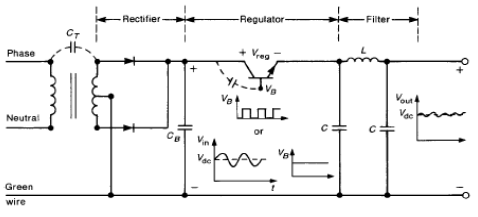
\includegraphics[width=0.45\linewidth]{immagini/emissioni_condotte10}
    \end{figure}
    \item \textbf{Alimentatori switching}: impiegano interruttori (MOS) fatti commutare periodicamente a frequenze dei kHz. Garantiscono efficienze superiori al $90\%$, ma generano intensi disturbi condotti dovuti alle elevate derivate temporali di tensione ($dv/dt$) e di corrente ($di/dt$) associate alle rapide transizioni di commutazione.
    \begin{figure}[H]
    	\centering
    	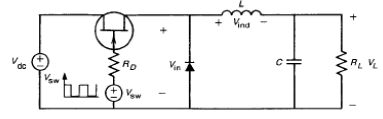
\includegraphics[width=0.45\linewidth]{immagini/emissioni_condotte11}
    \end{figure}
\end{itemize}

Nel \textbf{convertitore flyback}, ampiamente impiegato per alimentatori di rete, la transizione dell'interruttore MOSFET è controllata dalla tensione applicata al gate tramite un resistore $R_G$: 
\begin{figure}[H]
	\centering
	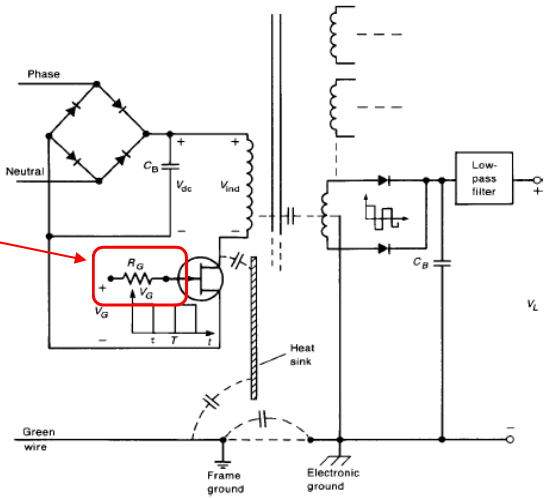
\includegraphics[width=0.5\linewidth]{immagini/emissioni_condotte12}
\end{figure}
Il \textbf{dimensionamento di $R_G$} stabilisce un compromesso tra efficienza ed emissioni elettromagnetiche:
\begin{itemize}
    \item Incremento di $R_G$ $\rightarrow$ rallenta i processi di carica e scarica della capacità di ingresso del MOSFET, riducendo le derivate $dv/dt$ e $di/dt$; i fronti di commutazione risultano addolciti e le emissioni condotte ad alta frequenza diminuiscono, ma aumenta il tempo trascorso dal dispositivo in zona attiva, incrementando le perdite di e abbassando il rendimento complessivo.
    \item Riduzione di $R_G$ $\rightarrow$ rende le transizioni di tensione e corrente estremamente ripide, riducendo al minimo le perdite e massimizzando l'efficienza energetica (fino a oltre il $95\%$), ma provoca una marcata iniezione di armoniche spettrali ad alta frequenza verso il telaio di terra.
\end{itemize}

Un secondo meccanismo di generazione del disturbo è legato ai \textbf{diodi raddrizzatori} d'uscita durante la fase di spegnimento. Quando la tensione applicata al diodo si inverte, le cariche immagazzinate nella regione di svuotamento della giunzione devono essere rimosse durante il \textit{tempo di recupero inverso}:
\begin{itemize}
    \item Nei dispositivi ad \textit{hard recovery}, la corrente inversa si interrompe con elevatissima pendenza ($di/dt$), innescando sovratensioni e oscillazioni risonanti ad alta frequenza che si propagano sulle linee di alimentazione.
    \item Nei dispositivi a \textit{soft recovery}, la corrente inversa decresce gradualmente verso lo zero, riducendo l'ampiezza delle oscillazioni transitorie.
    \item Per smorzare tali picchi, si inserisce in parallelo al diodo una \textit{rete snubber}, costituita dalla serie di un resistore $R$ e un condensatore $C$, che impone una costante di tempo di spegnimento controllata riducendo il contenuto armonico del disturbo di spegnimento.
\end{itemize}
\begin{figure}[H]
	\centering
	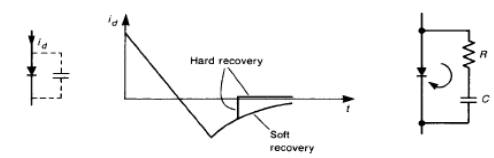
\includegraphics[width=0.6\linewidth]{immagini/emissioni_condotte13}
\end{figure}

Negli apparati reali, i percorsi di propagazione del disturbo sono determinati anche da altri accoppiamenti parassiti non intenzionali:
\begin{itemize}
    \item \textbf{Accoppiamento capacitivo tra transistor e dissipatore} $\rightarrow$ il MOSFET di potenza è montato a contatto meccanico con un dissipatore termico in alluminio. Tra la piastrina metallica del componente, soggetta a repentine variazioni di potenziale ($dv/dt$), e il corpo del dissipatore si instaura una capacità parassita $C_{\text{sink}}$. Se il dissipatore è collegato galvanicamente al telaio metallico di terra per ragioni di sicurezza, la corrente capacitiva ad alta frequenza:
    \[
    i = C_{\text{sink}} \frac{dv}{dt}
    \]
    scavalca l'isolamento circuitale e si inietta direttamente nel conduttore di protezione come corrente di modo comune.
    \begin{figure}[H]
    	\centering
    	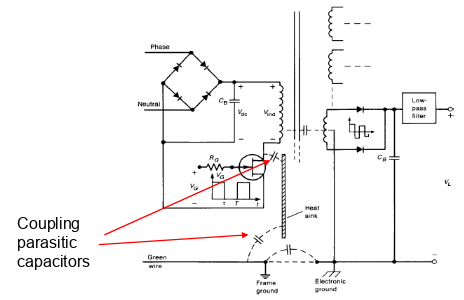
\includegraphics[width=0.6\linewidth]{immagini/emissioni_condotte14}
    \end{figure}
    
    \item \textbf{Accoppiamento capacitivo primario-secondario nel trasformatore} $\rightarrow$ sebbene il trasformatore garantisca l'isolamento galvanico, tra gli avvolgimenti primari e secondari è presente una capacità parassita distribuita $C_{PS}$. Alle alte frequenze, l'impedenza di $C_{PS}$ diventa sufficientemente bassa da consentire il trasferimento dei disturbi di commutazione dal circuito primario al secondario:
    \begin{figure}[H]
    	\centering
    	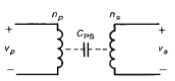
\includegraphics[width=0.3\linewidth]{immagini/emissioni_condotte15}
    \end{figure}
    Per interrompere l'accoppiamento capacitivo attraverso $C_{PS}$, tra l'avvolgimento primario e l'avvolgimento secondario viene interposta una lamina conduttrice di rame (schermo di Faraday). Lo schermo deve essere obbligatoriamente collegato alla massa del telaio; in tal modo la capacità $C_{PS}$ si scompone in due capacità parassite distinte, $C_{PF}$ tra primario e schermo e $C_{FS}$ tra schermo e secondario, e le correnti parassite generate dal primario vengono drenate a terra dallo schermo senza raggiungere l'avvolgimento secondario.
    \begin{figure}[H]
    	\centering
    	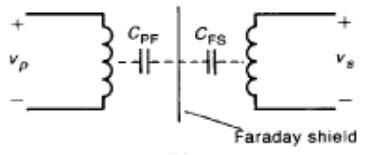
\includegraphics[width=0.3\linewidth]{immagini/emissioni_condotte16}
    \end{figure}
\end{itemize}

\section{Filtro per l'alimentazione}
La tensione utile a $50\text{ Hz}$ non può essere alterata, mentre il rumore di commutazione si colloca nell'intervallo $150\text{ kHz} - 30\text{ MHz}$; l'abbattimento delle emissioni condotte richiede pertanto l'inserimento di un filtro passa-basso tra l'EUT e la LISN.

Il \textbf{posizionamento fisico del filtro} all'interno dell'involucro dell'apparato costituisce un vincolo di installazione critico:
\begin{itemize}
    \item Posizionamento corretto $\rightarrow$ il filtro deve essere montato più vicino possibile alla presa di alimentazione; in questo modo i conduttori non filtrati rimangono confinati all'interno del telaio e i cavi uscenti trasportano unicamente segnali depurati dai disturbi.
    \item Posizionamento non corretto $\rightarrow$ l'installazione del filtro in prossimità dell'alimentatore e a distanza dalla parete esterna lascia una tratta di cavo interno non schermata che agisce da antenna e i campi irradiati dai circuiti interni si riaccoppiano sui conduttori d'uscita a valle del filtro, bypassandone completamente l'azione.
\end{itemize}
\begin{figure}[H]
	\centering
	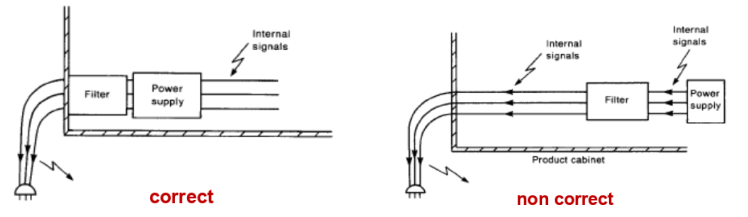
\includegraphics[width=0.7\linewidth]{immagini/emissioni_condotte17}
\end{figure}

La \textbf{topologia di un filtro di alimentazione} comprende quattro categorie di componenti:
\begin{figure}[H]
	\centering
	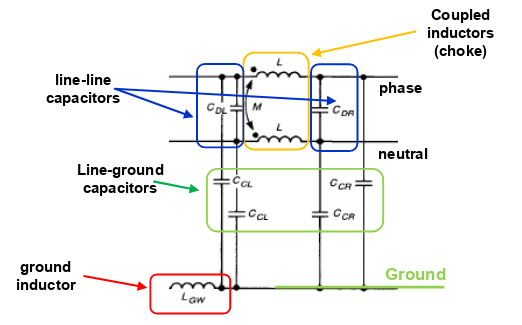
\includegraphics[width=0.7\linewidth]{immagini/emissioni_condotte18}
\end{figure}
\begin{itemize}
    \item \textbf{Condensatori line-line $C_D$} $\rightarrow$ collegati direttamente tra fase e neutro con valori tipici compresi tra $0.1\ \mu\text{F}$ e $0.47\ \mu\text{F}$. Forniscono un percorso a bassa impedenza che cortocircuita le correnti di modo differenziale.
    \item \textbf{Condensatori line-ground ($C_C$)} $\rightarrow$ collegati tra ciascun conduttore attivo e la massa metallica con valori tipici compresi tra $1000\text{ pF}$ e $4700\text{ pF}$ (ad esempio $3300\text{ pF}$). Drenano a terra le correnti di modo comune. Il valore massimo ammissibile è severamente vincolato dalle normative di sicurezza elettrica per limitare la corrente di dispersione verso terra a $50\text{ Hz}$ entro soglie non pericolose per l'utente in caso di interruzione accidentale del $C_DL$conduttore di protezione.
    \item \textbf{Induttore sul conduttore di protezione ($L_{GW}$)} $\rightarrow$ induttore inserito in serie sulla linea di terra con valore tipico di $1\text{ mH}$; incrementa l'impedenza del percorso di ritorno a massa ad alta frequenza ostacolando la circolazione del modo comune.
    \item \textbf{Choke a modo comune} $\rightarrow$ induttore realizzato avvolgendo simmetricamente due bobine identiche di induttanza $L$ su un unico nucleo toroidale in ferrite ad alta permeabilità, inserite in serie sulle linee di fase e di neutro con polarità concordi rispetto alla corrente uscente.
    \begin{figure}[H]
    	\centering
    	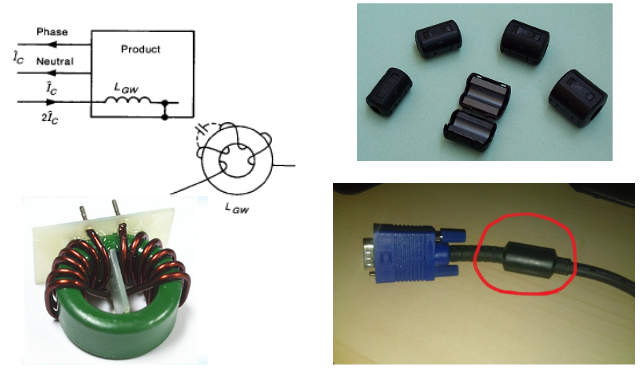
\includegraphics[width=0.5\linewidth]{immagini/emissioni_condotte19}
    \end{figure}
\end{itemize}

Il funzionamento del choke a modo comune si basa sulla cancellazione o sulla somma dei flussi magnetici indotti nel nucleo:
\begin{itemize}
    \item Funzionamento per il modo differenziale $\rightarrow$ le correnti di modo differenziale $\hat{I}_D$ attraversano i due avvolgimenti in versi opposti. I flussi magnetici generati nel nucleo toroidale possiedono verso contrario e si elidono reciprocamente. Assumendo un coefficiente di accoppiamento unitario:
    \[
    k = \frac{M}{L} \approx 1 \implies M \approx L
    \]
    la caduta di tensione complessiva ai capi dell'avvolgimento vale:
    \[
    \hat{V} = i\omega L \hat{I}_D - i\omega M \hat{I}_D = i\omega(L - M)\hat{I}_D \approx 0
    \]
    L'induttanza effettiva coincide con la sola induttanza di dispersione residua $L_{\text{dispersione}} = L - M$, dell'ordine di grandezza dei microhenry. Di conseguenza, il componente non introduce cadute di tensione apprezzabili né sulla corrente di carico a $50\text{ Hz}$ né sulle componenti differenziali.
    \begin{figure}[H]
    	\centering
    	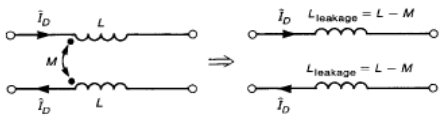
\includegraphics[width=0.45\linewidth]{immagini/emissioni_condotte20}
    \end{figure}
    \item Funzionamento per il modo comune $\rightarrow$ le correnti di modo comune $\hat{I}_C$ scorrono in entrambi gli avvolgimenti nello stesso verso. I flussi magnetici indotti nel nucleo si sommano costruttivamente. La tensione ai capi di ciascun avvolgimento vale:
    \[
    \hat{V} = i\omega L \hat{I}_C + i\omega M \hat{I}_C = i\omega(L + M)\hat{I}_C \approx i\omega(2L)\hat{I}_C
    \]
    Il choke manifesta un'induttanza apparente pari a circa il doppio dell'induttanza di singolo avvolgimento, a cui si associa la resistenza dissipativa per perdite nel materiale ferromagnetico $R(f)$, realizzando un blocco in serie ad alta impedenza per il modo comune.
    \begin{figure}[H]
    	\centering
    	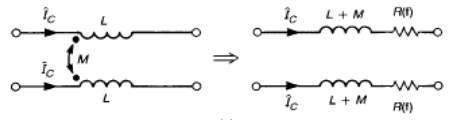
\includegraphics[width=0.45\linewidth]{immagini/emissioni_condotte21}
    \end{figure}
\end{itemize}
Manicotti cilindrici in ferrite: elementi di ferrite applicati esternamente attorno a cavi schermati o fasci conduttori (quali i cavi video o di alimentazione esterna); funzionano come induttori a spira singola introducendo un'impedenza serie di modo comune con marcate proprietà dissipative per smorzare i disturbi condotti guidati.

L'\textbf{analisi del filtro} si esegue per mezzo di due circuiti equivalenti:
\begin{itemize}
    \item Circuito equivalente di modo comune $\rightarrow$ le sorgenti di rumore sono rappresentate da due generatori di corrente $\hat{I}_C$ iniettati simmetricamente su fase e neutro rispetto a massa. I nodi di fase e neutro si trovano allo stesso potenziale, pertanto, la corrente che attraversa i condensatori linea-linea $C_{DL}$ e $C_{DR}$ è nulla. Il modello disaccoppiato comprende:
    \begin{itemize}
        \item Sorgente di corrente $\hat{I}_C$.
        \item Condensatore verso massa lato carico $C_{CR}$ in parallelo alla sorgente.
        \item Induttanza serie di modo comune $(L + M)$ lungo il conduttore attivo.
        \item Induttanza di terra raddoppiata $2L_{GW}$ lungo il ramo di ritorno di massa.
        \item Condensatore verso massa lato rete $C_{CL}$ in parallelo al carico di misura.
        \item Resistenza di misura da $50\ \Omega$ della LISN su cui si sviluppa la tensione di modo comune $\hat{V}_C$.
    \end{itemize}
    \begin{figure}[H]
    	\centering
    	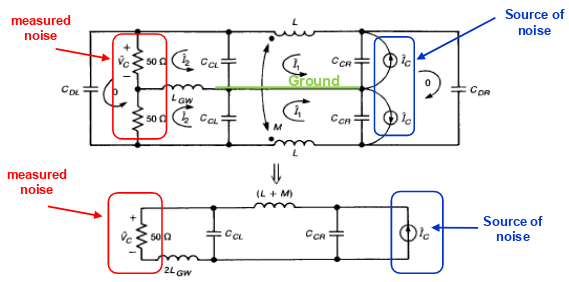
\includegraphics[width=0.7\linewidth]{immagini/emissioni_condotte22}
    \end{figure}
    \item Circuito equivalente di modo differenziale $\rightarrow$ le sorgenti di disturbo sono modellate da generatori in opposizione $\hat{I}_D$. Per antisimmetria, il potenziale sul conduttore di protezione di terra è nullo lungo l'intero asse; pertanto, nessuna corrente di modo differenziale scorre attraverso l'induttore di terra $L_{GW}$. Ciascun condensatore linea-linea collegato tra fase e neutro si sdoppia nel circuito equivalente di modo differenziale in una capacità di valore doppio ($2C_{DR}$ e $2C_{DL}$) posta in parallelo ai condensatori verso massa. Il modello disaccoppiato comprende:
    \begin{itemize}
        \item Sorgente di corrente $\hat{I}_D$.
        \item Parallelo capacitivo formato da $C_{CR}$ e $2C_{DR}$ lato carico.
        \item Induttanza serie di dispersione $(L - M)$ lungo la linea attiva.
        \item Ramo di ritorno privo di impedenze induttive.
        \item Parallelo capacitivo formato da $C_{CL}$ e $2C_{DL}$ lato rete.
        \item Resistenza di misura da $50\ \Omega$ della LISN su cui si sviluppa la tensione differenziale $\hat{V}_D$.
    \end{itemize}
    \begin{figure}[H]
    	\centering
    	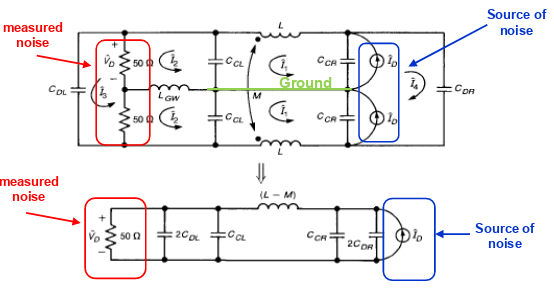
\includegraphics[width=0.7\linewidth]{immagini/emissioni_condotte23}
    \end{figure}
\end{itemize}

La seguente analisi mostra l'abbattimento delle componenti di rumore man mano che i singoli elementi del filtro vengono aggiunti al circuito:
\begin{enumerate}
	\item Circuito Senza Filtro $\rightarrow$ Lo spettro di rumore totale (dato dalla combinazione di DM a basse frequenze e CM ad alte frequenze) supera ampiamente la linea di limite normativo CISPR 22 Classe	B.
	\begin{figure}[H]
		\centering
		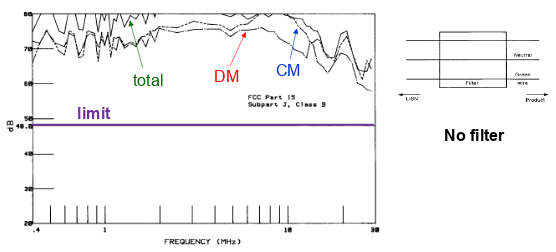
\includegraphics[width=0.57\linewidth]{immagini/emissioni_condotte24}
	\end{figure}
	\item Inserimento Condensatori Line-to-Ground (3300 pF) $\rightarrow$ Introducono una frequenza di taglio a circa 1 MHz. Il rumore di Modo Comune viene abbattuto drasticamente per f >> 1 MHz, ma la componente di Modo Differenziale a bassa frequenza rimane al di sopra del limite.
	\begin{figure}[H]
		\centering
		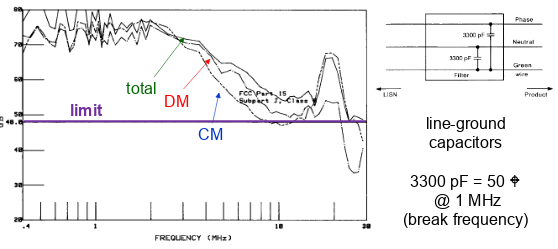
\includegraphics[width=0.57\linewidth]{immagini/emissioni_condotte25}
	\end{figure}
	\item Inserimento Condensatore Line-to-Line (0.1 $\mu$F) $\rightarrow$ Fissa una frequenza di taglio a 15.7 kHz.
	La componente di Modo Differenziale crolla per frequenze f >> 16 kHz, portando il rumore DM sotto
	la maschera.
	\begin{figure}[H]
		\centering
		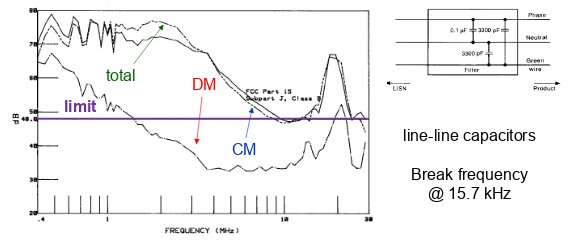
\includegraphics[width=0.6\linewidth]{immagini/emissioni_condotte26}
	\end{figure}
	\item Inserimento Induttore di Terra (1 mH) $\rightarrow$ Introduce una frequenza di taglio a 4 kHz,
	riducendo ulteriormente il Modo Comune nelle zone spettrali intermedie.
	\begin{figure}[H]
		\centering
		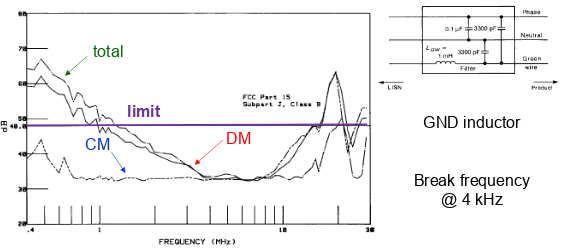
\includegraphics[width=0.6\linewidth]{immagini/emissioni_condotte27}
	\end{figure}
	
	\item Inserimento del Common Mode Choke $\rightarrow$ Abbatte le residue creste spettrali di Modo Comune,
	garantendo che l'intero spettro di emissione rientri al di sotto della maschera limite con un margine
	di sicurezza adeguato.
	\begin{figure}[H]
		\centering
		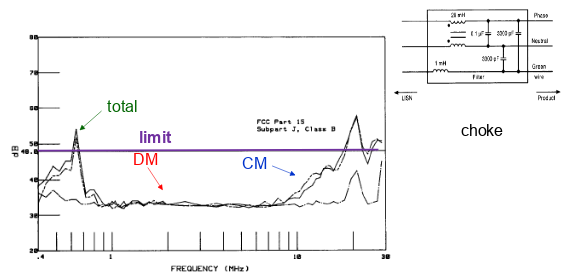
\includegraphics[width=0.6\linewidth]{immagini/emissioni_condotte28}
	\end{figure}
\end{enumerate}

